\chapter{Introduction to Condensed Matter Physics}
\section{What Is Condensed Matter Physics?}

``Condensed matter physics is the field of physics that deals with the macroscopic and microscopic physical properties of matter. In particular, it is concerned with the "condensed" phases that appear whenever the number of constituents in a system is extremely large and the interactions between the constituents are strong. The most familiar examples of condensed phases are solids and liquids, which arise from the electromagnetic forces between atoms.''
\section{Diffraction of Waves by Crystal}
We study crystal structure through the diffraction of photons, neutrons, and electrons . The diffraction depends on the crystal structure and on the wavelength. The atomic structure of crystalline solids is commonly determined using one of several different X-ray diffraction techniques. Complementary structure information can also be obtained through electron and neutron diffraction. In all instances, the radiation used must have wavelengths in the range of $0.1$ to $10 $\AA  \ because the resolution (or smallest object separation distance) to which any radiation can yield useful information is about equal to the wavelength of the radiation, and the average distance between adjacent
atoms in solids is about $10^{ -10}  $m  (1 \AA).
\subsection{Bragg's Law}
We consider the interference effects of X-rays when scattered by the atoms, comprising a crystal lattice. This is analogous to studying the structure of an optical diffraction grating by examining the interference pattern produced when we shine visible light on the grating. (The spacing of lines on a grating is about $0.5$ to $1 \mu \mathrm{m}$ and the wavelength of visible radiation ranges from $0.4$ to $0.8 \mu \mathrm{m}$.) In the optical grating the ruled lines act as scattering centers, whereas in a crystal it is the atoms (more correctly, the electrons about the atom) which scatter the incident radiation.
\begin{figure}[H]
	\centering
	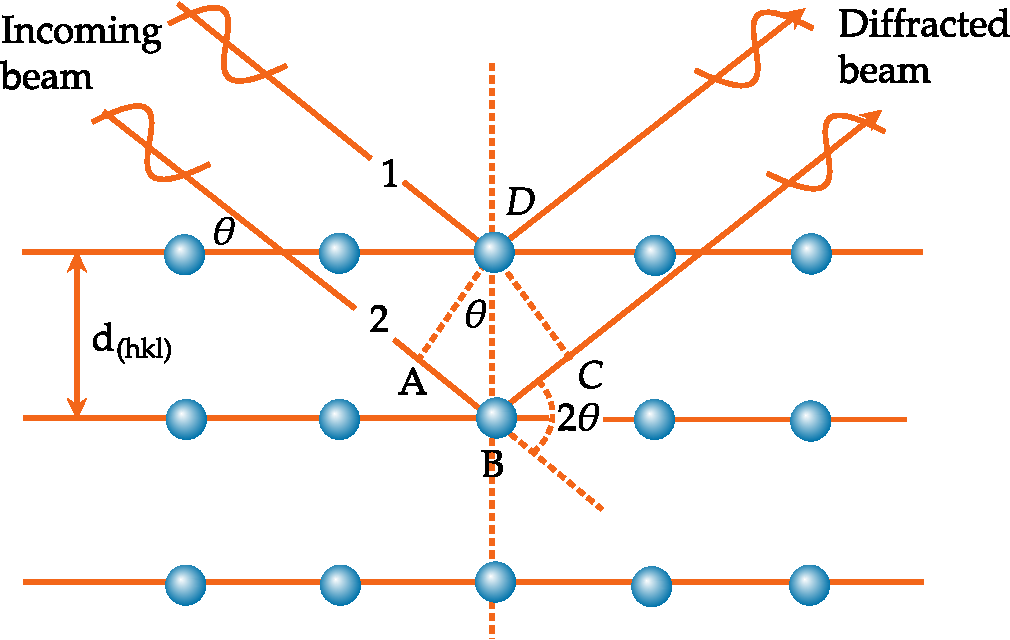
\includegraphics[height=4.9cm,width=8cm]{xray diffraction}
	\caption{Bragg's law, assuming the planes of atoms behave as reflecting planes.}
	\label{Bragg's law}
\end{figure}
\begin{equation}
d_{(h k l)}=\frac{a}{\sqrt{h^{2}+k^{2}+l^{2}}}
\end{equation}
For constructive interference of the scattered X-rays (the appearance of a diffraction peak) it is required that the beams, scattered on successive planes, be "in phase" (have again a common wave front) after they leave the surface of the crystal. In terms of the beams labeled 1 and 2 in figure. \ref{Bragg's law} this requires that the distance $\overline{\mathrm{AB}}+\overline{\mathrm{BC}}$ be equal to an integral number of wavelengths $(\lambda)$ of the indicent radiation. Accordingly:

\begin{align}
\overline{\mathrm{AB}}+\overline{\mathrm{BC}}&=\mathrm{n} \lambda \quad(\mathrm{n}=1,2,3, \ldots) \\
\text { Since } \overline{\mathrm{AB}}&=\overline{\mathrm{BC}} \text { and } \sin \theta=\frac{\overline{A B}}{d_{(h k)}}\quad \left[\overline{A B}=d_{(h k l)} \sin \theta\right] \\
n \lambda&=2 d_{(h k l)} \sin \theta
\end{align}
This relation is referred to as Bragg’s law and describes the angular position of the
diffracted beam.
